\documentclass[13pt]{article}
\usepackage[francais]{babel}
\usepackage[utf8]{inputenc}
\usepackage[T1]{fontenc}

\usepackage{verbatim}
\usepackage{amsthm}
\usepackage{amsmath,amssymb,amstext}
\usepackage{thmbox}
\usepackage{fancyhdr}
\usepackage{graphicx}
\usepackage{wrapfig}
\usepackage{url}


\newtheorem{bin}{ \textbf{Logique Binaire} }
\newtheorem{arit}{ \textbf{Arithmétique} }
\newtheorem{instr}
{ \textbf{Instructions actuellement prises en charges} }
\newtheorem{instrFutures}
{ \textbf{Instructions à venir} }

\newcommand{\cg}{[\kern-0.15em [}
\newcommand{\cd}{]\kern-0.15em ]}

\pagestyle{fancy}
\rhead{}

\title{Rapport du Projet de Système digital \no3}
\author{Belghiti Ismael, Desfontaines Damien, Geoffroy Guillaume, Maillard Kenji}
\date{\today}

\begin{document}
\renewcommand{\labelitemi}{$\triangleright$}

\maketitle
\tableofcontents
\newpage
\section{Introduction}
Le projet du cours de systéme digital a pour but de programmer une horloge en
assembleur, cette horloge devant tourner sur un processeur simulé en tant que
circuit digital synchrone sur un ordinateur. Notre approche du problème consiste
à encoder les circuits dans un langage nommé \emph{Rock}, puis de le compiler
avec \emph{Obsidian}, de coder un microprocesseur suivant la spécification de
l'architecture MIPS en Rock, de coder l'horloge en assembleur MIPS, d'assembler
ce code MIPS avec un assembleur fabriqué par nos soins et enfin de charger ce
dernier résultat dans le microprocesseur.\\
On présentera d'abord le langage rock, avant de s'intéresser à l'implémentation
du compilateur, du microprocesseur, de l'assembleur, puis de l'horloge. La
dernière partie contient des informations importantes pour l'utilisation en
pratique de ce que nous avons produit. 


\section{Le langage rock}

Le langage de description des circuits est un langage déclaratif basé sur la
notion de bloc. Nous l'avons appelé \emph{rock}. Il y a trois types de blocs différents :
\begin{itemize}
\item Les blocs de base : xor, and, or, mux, not, ground, vdd et reg (déclarés dans Analysis/baseBlocks.ml)
\item Les blocs déclarés par l'utilisateur, qui peuvent être paramétrés par des
entiers. Les entrées et les sorties de ces blocs sont des fils, et le corps des
blocs est déterminé à partir de blocs plus petits précédemment déclarés. 
\item Les périphériques ou blocs externes.
\end{itemize}

Il est compilé à l'aide du logiciel \emph{obsidian} dont l'organisation est
schématisée dans la figure 1. Les sections suivantes présentent les aspects spécifiques du langage et de sa compilation.

\subsection{Traitement lexical}
Le langage contient deux mots clés {\bf start} et {\bf device } ainsi que les
caractères {\bf <}, {\bf >}, {\bf (}, {\bf )}, {\bf $\to$}, {\bf ;}, {\bf :}, {\bf ,},
{\bf [}, {\bf ]}, {\bf \{}, {\bf \}}, {\bf .}, {\bf ..}, {\bf +}, {\bf -}, {\bf *}, {\bf /},
{\bf \%}, {\bf \^{}}, {\bf @}. 

Les identifiants sont de l'une des deux formes suivantes :
\begin{description}
\item[NomBloc : ] un identifiant commençant par une majuscule, il sert à
  identifier les blocs et les variables de blocs.
\item[NomFil : ] identifiant commençant par une minuscule, il sert à identifier
  les noms de fils et de variables entières.
\end{description}

L'opération d'analyse lexicale se charge aussi d'effacer les commentaires qui
sont soit de la forme \og $(*$\fg{} \og $*)$\fg{} pour les commentaires
multi-lignes, soit de la forme \og \#\fg{} pour les commentaires sur une seule ligne.

\begin{figure}
  \begin{center}
    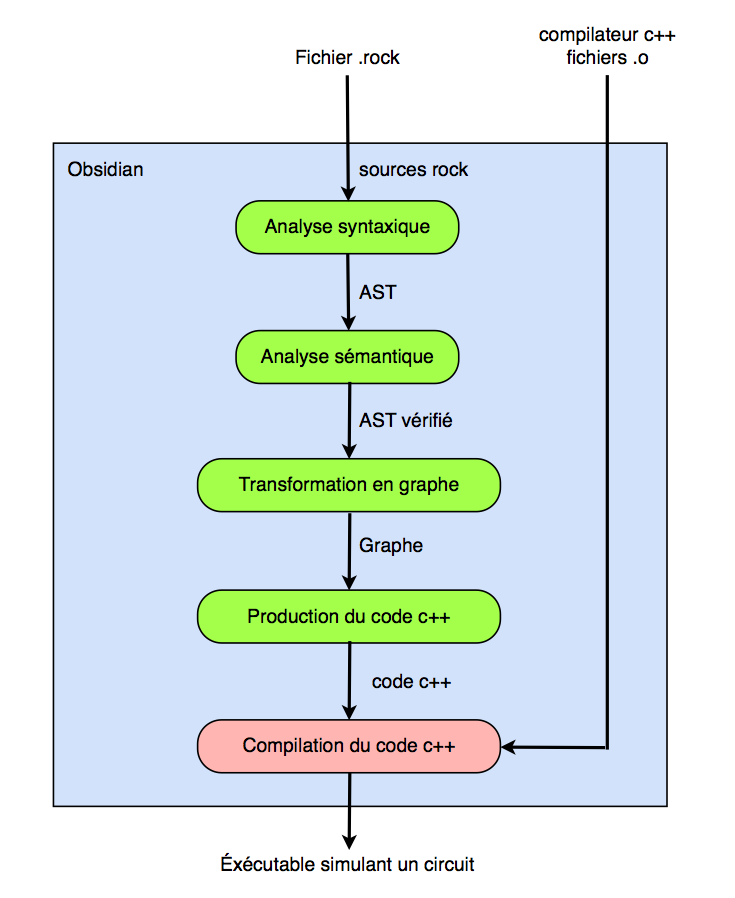
\includegraphics[width=14.7cm,height=17.96cm]{obsidian.png}
    \caption{Architecture d'Obsidian}
    \label{Architecture d'Obsidian}
  \end{center}
\end{figure}

\subsection{Syntaxe du langage}
Le langage suit la grammaire suivante :\newline\newline
\begin{tabular}{ r c l }
  fichier &$::=$&\: instruction* BlocEntrée instruction*\\ [1.5ex]
  BlocEntrée &$::=$&\: {\bf start} NomBloc $<$ ConstanteEntière, ... ,
  ConstanteEntière  $>$\\ [1.5ex]
  instruction &$::=$&\: BlocDéfinition\\
  &&| PériphériqueDéfinition \\ [1.5ex]
  BlocDéfinition &$::=$&\: NomBloc Paramètres? Arguments? Instance* $\to$
  Sorties $;$\\ [1.5ex]
  PériphériqueDéfinition &$::=$&\: {\bf device} NomBloc Paramètres\\ [1.5ex]
  Paramètres &$::=$&\: $<$ Motif, ... , Motif $>$\\ [1.5ex]
  Motif &$::=$&\: $a*n+k+b$     \\ 
  &&| $a*n+b$  \\ 
  &&| $b$ \\ 
  \multicolumn{3}{c}{(avec $a$, $b$ des constantes entières, $a
    \neq 1$ et $n$, $k$ des identifiants de variables)} \\ [1.5ex]
  Arguments &$::=$&\: $($ DeclarationFil, ... , DeclarationFil $)$ \\ [1.5ex]
  DeclarationFil  &$::=$&\: NomFil \\
  &&| NomFil $[$ ConstanteEntière $]$ \\ [1.5ex]
 
  Instance &$::=$&\: NomBloc NomVariableBloc $($ Fil, ... , Fil $)$ \\ [1.5ex]
  Fil &$::=$&\: NomFil\\
  &&| NomVariableBloc {\bf .} NomFil\\
  &&| NomFil $[$ ConstanteEntière $]$\\
  &&| NomFil $[$ ConstanteEntière {\bf..} ConstanteEntière $]$\\
  &&| {\bf \$} $(0|1)+$ \\
  &&| $\mathbf{\{}$ Fil, ... , Fil $\mathbf{\}}$\\ [1.5ex]
  Sorties&$::=$&\: DeclarationFil : Fil, ... , DeclarationFil : Fil
\end{tabular}
\text{}\\

\subsection{Principe des blocs}
Les blocs sont les unités structurantes du langage. Ils sont séparés en 3
catégories :
\begin{itemize}
\item Les blocs de base qui sont fournis par le compilateur ( \texttt{Xor}, \texttt{And}, \texttt{Reg},
  \texttt{Mux}, \texttt{Vdd}, \texttt{Gnd}, etc).
\item Les blocs classiques qui définissent la majeure partie du circuit.
\item Les périphériques qui permettent d'introduire des éléments externe dans le langage.
\end{itemize}
\text{}\\
Les blocs classiqus se construisent par composition. Ils ont en général la forme
suivante : 
\begin{verbatim}
BlocDéfini < params > (arg1, ..., argn)
   Bloc1  Instance1(arg1', ... , argp')
   Bloc2  Instance2(arg1'', ... , argq'' )
   -> sortie1 : fil1, ... , sortiek : filk ;
\end{verbatim}


\subsection{Les entiers} 
Les constantes entières sont présentes dans les paramètres - pour permettre de
coder des blocs récusrivement - et dans les fils - pour pouvoir préciser leur taille.
\text{}\\

On peut les écrire tout aussi bien en hexadécimal (préfixe \og $0x$\fg{} ou \og $0X$\fg{}), en
octal (préfixe \og $0o$\fg{} ou \og $0O$\fg{}), en binaire (préfixe \og $0b$ \og
ou \og $0B$\fg{}) ou en décimal (sans préfixe).
Ils supportent les opérations suivantes :
\begin{itemize}
\item $+$ l'addition
\item $-$ la soustraction
\item $*$ le produit
\item $/$ le quotient (division euclidienne)
\item $\%$ le reste (division euclidienne)
\item \^{} l'exponentiation
\end{itemize}


\subsection{Les fils}

Les fils présents dans rock sont des fils épais. Ils sont les seuls moyens de
communication entre blocs. Ils sont passés en arguments lors de la construction
d'une instance et retournés à l'aide de la syntaxe \texttt{nom du bloc . nom du
  fil en sortie}.
Les fils supportent deux opérations :
\begin{itemize}
\item l'extraction d'un sous-fil se fait via la syntaxe $a[\ p\ ..\ q\ ]$ et crée
  un nouveau fil de largeur $q - p + 1$ qui est branché sur les fils sous-jacents
  de $a$ indicés de $p$ à $q$.
\item la fusion de fils se fait via la syntaxe $\{ a_1, a_2, ..., a_n \}$ et
  produit un fil dont la largeur est la somme des largeurs des $a_i$.
\end{itemize} 
\text{}\\
En plus de ces opérations, du sucre syntaxique a été rajouté pour améliorer
l'expérience utilisateur :
\begin{itemize}
\item La syntaxe $a[n]$ est équivalente à $a[n..n]$ et produit donc un fil de
  taille 1.
\item La syntaxe du type $\$01101$ est
  équivalente à :
\begin{verbatim}
    Gnd G
    Vdd V
    ... { G.o, V.o, V.o, G.o, V.o } ...
\end{verbatim}
  c'est à dire à un fil où chaque $1$ est remplacé par un fil portant toujours
  la valeur $1$ (instance de \texttt{Vdd}) et chaque $0$ par un fil portant
  toujours la valeur $0$ (instance de \texttt{Gnd}). 
\end{itemize}


\section{Concepts clés du langage}

Le langage rock est muni de plusieurs concepts qui en font un outil maniable,
utile, et efficace : citons notamment la récursion, les périphériques et les
redéfinitions locales d'horloges.

\subsection{Motifs et récursion}
Le langage ne dispose pas des boucles classiques (\texttt{for}, \texttt{while})
ni de structures conditionnelles (\texttt{if}) pour manipuler le flot d'exécution. Il est par
contre doté d'un système puissant de récursion et de reconnaissance de motifs.
Il y a deux types de motifs :
\begin{itemize}
\item les motifs constants qui n'acceptent que leur valeur. 
\item les motifs de la forme $ a*n + b $, avec $a$, $b$ constants et $n$
  variable, qui acceptent les entiers $p$  tels que $p \equiv b\
  \text{mod}\ a$ et on a alors $n = \frac{p - b}{a}$.
\item les motifs de la forme $ a*n + k + b $, avec $a \neq 1 $, $b$ constants et
  $k$, $n$ variables, qui acceptent tous les entiers $p$, et posent $k \equiv  p - b\
  \text{mod}\ a$, $0 \leq k < a$ et $n = \frac{p - b - k}{a}$.
\end{itemize}
\text{}\\
Étant donnés un entier $p$ et une liste ordonnée de motifs $(m_i)_i$, les motifs
fonctionnent selon le principe suivant : 
\begin{itemize}
\item l'entier est testé sur le $i^{e}$motif (en prenant au départ $i=0$),
\item s'il est accepté, les variables correspondant au motif sont assignées si
  nécessaire,
\item et s'il est rejeté, on passe au motif suivant et on recommence.
\end{itemize}
Si on ne trouve aucun motif convenable, le compilateur lève une erreur.
\text{}\\
\text{}\\
Un tel système de motifs permet différents types de récursions. Ainsi, on peut :
\begin{itemize}
\item itérer sur tous les entiers avec les motifs $<n+1>$ et $<0>$,
\item itérer seulement sur les puissances de deux avec les motifs $<2*n>$ et $<1>$,
\item ou encore travailler sur des congruences modulo 3 avec les motifs $<3*n>$, $<3*n +
  1>$ et $<3*n + 2>$.
\end{itemize}
\text{}\\
Ce système est néanmoins sujet à des limitations théoriques : il faut s'assurer
que les calculs et la compilation se terminent ; et notamment qu'il n'y a pas de
chaîne infinie de blocs. Pour cela, une contrainte supplémentaire a été ajoutée
: à l'intérieur d'un bloc ayant comme paramètres les entiers $(n_i)_i$, seuls
des blocs avec des paramètres plus petits (au sens de l'ordre sur
$\mathfrak{N}$) peuvent être instanciés.

\subsection{Les périphériques}


Les périphériques sont un moyen de définir de nouvelles portes en plus des
portes de base. On peut les utiliser pour simuler des mémoires, ou des
périphériques d'entrée/sortie.

Tous les périphériques ont la même interface (les mêmes fils d'entrée et
les mêmes fils de sortie) :
\begin{itemize}
\item Entrée :
\text{}\\
\begin{center}
  \begin{tabular}{ | c | c | }
    \hline
    Address &  32 bits \\
    \hline
    Data & 32 bits \\
    \hline
    Write mode & 1 bit\\
    \hline
    Byte enables &  4 bits\\
    \hline
    Enable interrupt & 1 bit\\
    \hline
    Interrupt processed & 1 bit\\
    \hline
  \end{tabular}
\end{center}
\text{}\\
\item Sortie :
\text{}\\
\begin{center}
 \begin{tabular}{ | c | c | }
    \hline
    Data &  32 bits \\
    \hline
    Interrupt request & 1 bit \\
    \hline
  \end{tabular}
\end{center}
\end{itemize}
\text{}\\
Les périphériques peuvent contenir du code arbitraire, et peuvent donc a
priori gérer leurs entrées et sorties de n'importe quelle
manière. Cependant, ils sont faits pour simuler des périphériques mappés en
mémoire : Les entrées \texttt{Address}, \texttt{Data} et \texttt{Write mode} et
la sortie \texttt{Data} 
fonctionnent comme leur nom l'indique (l'entrée \texttt{Data} contient les données
à écrire si \texttt{Write mode} $=  1$, la sortie \texttt{Data} contient les données lues).
L'entrée \texttt{Byte enables} indique quels octets il faut prendre en compte :
\begin{itemize}
\item   Si à l'adresse $0$ se trouve la suite d'octets $11\ 22\ 33\ 44$, et si l'on
    essaye de lire à l'adresse $0$ avec \texttt{Byte enables} = $\$1010$, la valeur lue
    correspondra à la suite d'octets $11\ 00\ 33\ 00$.

\item  Si à l'adresse $0$ se trouve la suite d'octets $11\ 22\ 33\ 44$, et si l'on
    essaye d'écrire $55\ 66\ 77\ 88$ à l'adresse $0$ avec \texttt{Byte enables} $= \$1010$,
    on trouvera à l'adresse $0$ la suite d'octets $55\ 22\ 77\ 44$.
\end{itemize}

Les périphériques sont pensés comme des registres, c'est-à-dire que si l'on
écrit l'adresse où l'on veut lire au cycle t, on pourra lire le résultat au
cycle t+1. A posteriori, il aurait été plus pratique de donner le choix
entre les deux modes de fonctionnement (lecture instantanée et lecture
retardée d'un cycle), car lorsqu'un périphérique n'est pas utilisé pour
couper une boucle combianatoire, on perd simplement un cycle à attendre.

On déclare les types de périphériques de la façon suivante :

\begin{verbatim}
  device Memory<size>
\end{verbatim}

Puis, le type de périphérique peut être instancié comme n'importe quel
autre type de bloc, par exemple, le circuit suivant :
\begin{verbatim}
  Start
      Memory<5> Ram($0000...0000, $0000...0000, $1111, $0, $0)
      -> out[32] : Ram.dtata;

  start Start
\end{verbatim}
est constitué d'une mémoire sur $2^5 = 32$ octets, et sa sortie correspond au
mot de $32$ bits contenu à l'adresse $0$ dans la mémoire. Si la mémoire est
prévue pour initialiser tous ses octets à $0$, la sortie de ce circuit sera :

\begin{verbatim}
  00000000000000000000000000000000
  00000000000000000000000000000000
  00000000000000000000000000000000
  00000000000000000000000000000000
  ...
\end{verbatim}

Et le circuit suivant :

\begin{verbatim}
  Start
      Memory<5> Ram($0000...0000, $1111...1111, $1100, $1, $0)
      -> out[32] : Ram.dtata;

  start Start
\end{verbatim}

Aura pour sortie :

\begin{verbatim}
  00000000000000000000000000000000
  11111111111111110000000000000000
  11111111111111110000000000000000
  11111111111111110000000000000000
  ...
\end{verbatim}

On définit les types périphériques de la manière suivante :
Chaque type de périphérique est défini par une classe C++, qui doit
hériter de la classe device :
\begin{verbatim}
  class device
  {
  public :
    virtual ~device();
    virtual unsigned int cycle (unsigned int address, unsigned int data,
                                char byte_enables, bool write_enable,
                                bool interrupt_enable, bool iack, char *
                                irq)=0;
  };
\end{verbatim}
Chaque périphérique doit également fournir une méthode statique \texttt{make}, qui
construit un objet de cette classe et renvoie un pointeur vers cet objet,
upcasté en \texttt{device*}. Cette méthode prend un argument (de type \texttt{int}) par
paramètre du périphérique. Par exemple, pour le périphérique \texttt{Memory}, la
méthode \texttt{make} a le prototype suivant :

\begin{verbatim}
  device * make (int size)
\end{verbatim}

Pour chaque périphérique du circuit, sa méthode \texttt{cycle} est appelée à
chaque cycle, avec comme arguments les valeurs lues dans les fils d'entrée.


\subsection{Les enables}

Les enables permettent de redéfinir localement l'horloge du circuit :
le circuit suivant :
\begin{verbatim}
  Count_mod_2
      Not N(R.o)
      Reg R(N.o)
      -> o : R.o ;

  Start
      Count_mod_2 C1
      Count_mod_2 @ C1.o C2
      -> o : C2.o ;

  start Start
\end{verbatim}

contient deux compteurs modulo 2 : C1 et C2, mais à l'intérieur du second,
l'horloge est localement redéfinie, de sorte que le second compteur n'est
actif qu'au cycles où la sortie du premier vaut 1, c'est-à-dire un cycle
sur deux. La sortie du circuit est donc :

\begin{verbatim}
  0
  0
  1
  1
  0
  0
  1
  1
  ...
\end{verbatim}
Lorsqu'une porte n'est pas active, le code C++ correspondant n'est
simplement pas exécuté : la sortie de la porte garde sa valeur du cycle
précédent, et s'il s'agit d'un registre, son contenu n'est pas
modifié. Dans le cas d'un périphérique, sa méthode \texttt{cycle} n'est pas
appelée.


Si on redéfinit l'horloge d'un bloc, on redéfinit l'horloge de toutes les
portes et de tous les blocs qu'il contient. Si ce bloc lui-même redéfinit
l'horloge de l'un de ses composants, celui-ci ne sera actif que lorsque son
bloc parent l'est et que son bloc parent l'active. Par exemple, on peut
utiliser les enables pour programmer un compteur modulo $2^n$. Ainsi, le circuit
suivant :
\begin{verbatim}
  Count<1>
      Reg M(N.o)
      Not N(M.o)
      -> out : M.o,
         carry : M.o;

  Count<n>
      Count<1> Low
      Count<n-1> @ Low.carry High
      And A(Low.carry, High.carry)
      -> out[n] : {Low.out, High.out},
         carry : A.o;

  Start<n>
      Count<n> C
      -> out[n] : C.out;

  start Start<3>
\end{verbatim}
a pour sortie :
\begin{verbatim}
  000
  100
  010
  110
  001
  101
  011
  111
  000
  100
  010
  ...
\end{verbatim}

L'intérêt majeur des enables est qu'ils permettent de gagner du temps en
n'exécutant que les parties du circuit qui sont utiles au cycle en cours
(en plus de rendre certains codes plus simples, comme celui du compteur
modulo $2^n$). Par exemple, grâce aux enables, on peut définir un bloc
\texttt{Ram} de manière (à peu près) efficace :
\begin{verbatim}
  Mux_scalar <1> (selector, input0[1], input1[1])
      Mux M(selector, input0, input1)
      -> o : M.o;

  Mux_scalar <n> (selector, input0[n], input1[n])
      Mux_scalar<n-1> Low(selector, input0[0..n-2], input1[0..n-2])
      Mux High(selector, input0[n-1], input1[n-1])
      -> o[n] : {Low.o, High.o};

  Ram <0,1> (data[1], write)
      Mux M(write, R.o, data[0])
      Reg R(M.o)
      -> data[1] : R.o;

  Ram <0,d> (data[d], write)
      Ram<0,d-1> Low(data[0..d-2], write)
      Ram<0,1> High(data[d-1], write)
      -> data[d] : {Low.data, High.data};

  Ram <1,d> (address[1], data[d], write)
      Not N(address[0])
      Ram<0,d> @ address[0] Low(data, write)
      Ram<0,d> @ N.o        High(data, write)
      Mux_scalar<d> M(address, Low.data, High.data)
      -> data[d] : M.o;

  Ram <a,d> (address[a], data[d], write)
      Not N(address[a-1])
      Ram<a-1,d> @ N.o          Low(address[0..a-2], data, write)
      Ram<a-1,d> @ address[a-1] High(address[0..a-2], data, write)
      Mux_scalar<d> M(address[a-1], Low.data, High.data)
      -> data[d] : M.o;
\end{verbatim}
Ainsi, pour une mémoire de $2^a$ mots de $d$ bits, le temps de calcul pour un
cycle est en $O(a*d)$, au lieu du $O(2^a * d)$ que l'on aurait eu sans enables.


\subsection{Exemples de codes et de blocs classiques}
Voici quelques exemples de blocs que l'on peut définir avec ce langage :

\begin{verbatim}
### Manipulations de fils épais ###
\end{verbatim}

On peut effectuer diverses opérations sur les fils épais, par exemple le
renversement :

\begin{verbatim}
  Rev<1> (in[1])
      -> out[1] : in[0];

  Rev<n> (in[n])
      Rev<n-1> High(in[1..n-1])
      -> out[n] : {High.out, in[0]};
\end{verbatim}

On peut aussi étendre les opérations à des fils épais, bit-à-bit :

\begin{verbatim}
  And_vect<1> (a[1],b[1])
      And A(a[0],b[0])
      -> o : A.o;

  And_vect<n> (a[n],b[n])
      And Low(a[0],b[0])
      And_vect<n-1> High(a[1..n-1],b[1..n-1])
      -> o[n] : {Low.o, High.o};
\end{verbatim}

Ou à la manière d'un produit par un scalaire :

\begin{verbatim}
  And_scalar<1> (a,b[1])
      And A(a,b[0])
      -> o : A.o;

  And_scalar<n> (a,b[n])
      And Low(a,b[0])
      And_scalar<n-1> High(a,b[1..n-1])
      -> o[n] : {Low.o, High.o};
\end{verbatim}

Ou encore à la manière d'un fold :

\begin{verbatim}
  And_fold <1> (a[1])
      -> o : a;

  And_fold <n> (a[n])
      And_fold<n-1> Tail(a[0..n-2])
      And Head(a[n-1], Tail.o)
      -> o : Head.o;
\end{verbatim}
\begin{verbatim}
### Constantes ###
\end{verbatim}
On peut associer automatiquement à un entier n un fil épais représentant n
sur p bits :
\begin{verbatim}
  Bin<0,1>
      -> o : $0;
  Bin<1,1>
      -> o : $1;

  Bin<2*n,p>
      Bin<n,p-1> High
      -> o[p] : {$0, High.o};
  Bin<2*n+1,p>
      Bin<n,p-1> High
      -> o[p] : {$1, High.o};
\end{verbatim}
\begin{verbatim}
### Compteurs modulo n ###
\end{verbatim}
On peut tout d'abord définir un compteur modulo $2^{n}$ :
\begin{verbatim}
  Count<1> (enable)
      Reg R(X.o)
      Xor X(R.o,enable)
      And A(R.o,enable)
      -> out : R.o,
         carry : A.o;

  Count<n> (enable)
      Count<n-1> Low(enable)
      Count<1> High(Low.carry)
      -> out[n] : {Low.out, High.out},
         carry : High.carry;
\end{verbatim}
On peut aussi ajouter un argument "reset" au compteur :
\begin{verbatim}
  Count_reset<1> (e, r)
      Reg Mem(New_value.o)

      Not Not_reset (r)
      And New_value (Result.o, Not_reset.o)

      Xor Result(Mem.o,e)
      And Carry(Mem.o,e)
      -> o : Mem.o, c : Carry.o;

  Count_reset<n> (e, r)
      Count_reset<n-1> L(e, r)
      Count_reset<1> H(L.c, r)
      -> o[n] : {L.o, H.o}, c : H.c;
\end{verbatim}
Et à partir de là, on peut définir un compteur modulo n sur p bits :

Il faut d'abord définir une opération "égalité" sur des fils épais :
\begin{verbatim}
  Xor_vect<1> (a[1],b[1])
      Xor X(a[0],b[0])
      -> o : X.o;
  Xor_vect<n> (a[n],b[n])
      Xor Low(a[0],b[0])
      Xor_vect<n-1> High(a[1..n-1],b[1..n-1])
      -> o[n] : {Low.o, High.o};

  Not_vect<1> (a[1])
      Not N(a[0])
      -> o : N.o;
  Not_vect<n> (a[n])
      Not Low(a[0])
      Not_vect<n-1> High(a[1..n-1])
      -> o[n] : {Low.o, High.o};

  Is_equal<n> (a[n],b[n])
      Xor_vect<n> Not_equal(a,b)
      Not_vect<n> Equal(Not_equal.o)
      And_fold<n> All_equal(Equal.o)
      -> o : All_equal.o;
\end{verbatim}

Et le compteur :
\begin{verbatim}
  Counter<n,p> (e)
      Count_reset<p> C(e, Reset.o)
      Bin<n-1,p> Mod
      Is_equal<p> Reset(C.o,Mod.o)
      -> o[p] : C.o;
\end{verbatim}


\section{Spécificités techniques de l'implémentation d'Obsidian}

Le compilateur Obsidian s'occupe de transformer un fichier rock en éxécutable.
Il est codé en OCaml, langage trés partique pour la manipulation d'expression
symbolique, puis génére du code c++ qui est ensuite compilée par un compilateur
c++ classique pour tenter d'améliorer les performances. Dans la suite de cette
section, chaque étape est présentée avec ses particularités techniques et/ou
algorithmiques.

Les principales étapes du compilateur sont :
\begin{enumerate}
\item Le lexer et le parseur.
\item L'analyse sémantique.
\item La \og destruction \fg{} de l'AST en graphe.
\item La génération de code c++.
\end{enumerate}

\subsection{Le lexer et le parseur}

Les librairies ocamllex et menhir ont été employées pour faire cette partie. Les
symboles reconnus par le lexer ainsi que la grammaire employée dans le parser
ont déja été vus dans la présentation du langage. 

L'arbre de syntaxe abstraite (ou AST) est formé de la manière suivante :
\begin{itemize}
\item À la racine, d'un tableau associatif qui à chaque nom de bloc associe sa
  définition, d'une liste des périphériques déclarés avec leur nombre de
  paramètres ainsi que du nom et des paramètres du bloc de départ (celui qui
  englobe tout le circuit simulé).
\item Les définitions de blocs, sont des enregistrements dont les champs sont
  les paramètres du bloc (motifs), les entrées (fils), les instances (création
  de sous-bloc) et les sorties (fils). Ceux-ci sont eux même des types
  enregistrement jusqu'à arriver au atomes (nom de fil, nom de bloc, entier, etc).
\end{itemize}

L'AST, ou plutôt les AST, est paramétré par un module définissant les entiers à
utiliser dans l'AST (il s'agit donc d'un foncteur). L'intéret de paramétrer la
définition des entiers à l'intérieur de l'AST est de pouvoir produire à la
sortie du parser un AST dans lequel la plupart des \og entiers\fg{} sont en fait
des \emph{expressions entières} pas encore évaluées et qui seront transformées à
l'étape suivante.

\subsection{L'analyse sémantique}

L'analyse sémantique est un des morceaux les plus lourd d'Obsidian, mais aussi
ce qui fait du langage un outil utilisable car sur. En effet l'analyse statique
pratiquée au niveau de l'analyse sémantique permet d'éliminer presque toutes les
erreurs de sémantiques au niveau du circuit. Concrétement, l'analyse sémantique
vérifie :
\begin{itemize}
\item que tous les blocs employés ont été déclarés et que dans chaque blocs
  toutes les variables (que se soit de bloc ou de fil) ont été définis.
\item que tous les fils sont corrects c'est à dire qu'il n'y a jamais de fil
  vide voir d'épaisseur négative et que les branchements fait entre deux fils
  sont bien fait avec des fils de même largeur.
\item que chaque création de sous-fils ( avec la syntaxe $[\ ..\ ]$) est bien
  fait avec un intervalles valique (c'est à dire inclus dans l'intervalle $[| 0
  ; n - 1|]$ où $n$ est la taille du fil original).
\item que chaque applications de paramètres lors d'une instance est bien
  acceptée par un certain motif.
\item que la récursion est bien fondée, qu'il n'y a pas de suite infinie de
  blocs dans le circuit ce qui est une vérification cruciale pour l'étape de
  transformation en graphe. 
\end{itemize}

En particulier, l'analyse sémantique s'occupe d'une opération que l'on appelle
réification par analogie avec l'opération que font certains compilateurs pour
gérer le paramétrage polymorphique (par exemple avec les templates en c++). Il
s'agit en fait de transformer l'AST ne contenant que des entiers \og
formels\fg{} c'est à dire des \emph{expressions entières} en entiers.
Par exemple, le code suivant :
\begin{verbatim}
 And_vect<1> (a[1],b[1]) 
      And A(a[0],b[0])
      -> o : A.o;

  And_vect<n> (a[n],b[n])
      And Low(a[0],b[0])
      And_vect<n-1> High(a[1..n-1],b[1..n-1])
      -> o[n] : {Low.o, High.o};

  start And_vect<4>
\end{verbatim}

génére d'abord l'AST contenant les définitions de \texttt{And\_vect<1>} et
\texttt{And\_vect<n>}, puis aprés réification, il contiendra les définitions de
\texttt{And\_vect<1>}, \texttt{And\_vect<2>}, \texttt{And\_vect<2>},
\texttt{And\_vect<4>}. 

Cette multiplication de symboles peut paraître trés lourde mais elle permet une
analyse en détail de chaque blocs et l'étape suivante du compilateur fait
disparaître les redondances.

Il faut aussi noter que l'analyse sémantique ne vérifie pas l'absence totale de
cycle combinatoire. Pour cela, il faut attendre que l'AST soit transformé en
graphe. Il s'agit donc de la seule vérification doit attendre la phase de
génération de code pour être faite.

\subsection{La transformation en graphe}

À la sortie de l'analyse sémantique, un AST \emph{réifié} est obtenu. La
transformation en graphe se fait en deux étapes :
\begin{itemize}
\item Un premier parcours de l'AST pour déterminer la liste des portes
  que contiendra le graphe. Cette liste est ensuite transformée en tableau.
  Le choix des listes au début est pour permettre une concaténation efficace,
  tandis que la transformation en tableau à la fin est nécessaire pour avoir un
  accés aléatoire à chaque éléments.
\item Un deuxième parcours de l'AST se charge de \emph{brancher} les fils entre
  les portes. Pour cela on considère l'ensemble des \emph{bouts de fil} identifiables
  (c'est à dire l'ensemble des variables de fils en distinguant selon la portée)
  et on construit la relation d'équivalence \og est branché avec\fg{} avec un
  Union-find. Les classes d'équivalence résultantes à la fin du parcours sont
  exactement l'ensemble des fils.
\end{itemize}

Au passage, tous les blocs qui ne sont pas des blocs de base ou des
périphériques sont éliminés, ou plutôt oubliés, au cours de l'opération.
Le résultat est un graphe sous la forme d'un tableau où à chaque indice est
associé le type de la porte et un tableau contenant pour chaque sortie de la
porte en question les portes en aval avec lesquelles elle est branchée. Un
certain nombre d'informations telles que le nombre total de registres ou de
périphériques est aussi collecté durant cette phase pour aider la génération du code. 

\subsection{La génération du code c++}
vérification de l'absence de cycles combinatoires.
compilation vers du c++ pour les performances


\section{Le microprocesseur}

\section{L'assembleur}

Le microprocesseur lit en entrée du code éxécutable qui se trouve dans un
fichier \emph{ram} qu'il charge en mémoire. La génération du fichier \emph{ram}
à partir des sources MIPS incombe donc à l'assembleur. L'assembleur a été codé
sur la même architecture générale qu' Obsidian (lexer, parser, légére analyse
sémantique et génération du code) en OCaml. \\
La syntaxe du MIPS est assez simple à parser et à analyser, cependant quelques
limitations ont été introduites : 
\begin{itemize}
\item Il doit y avoir au plus une instruction ou étiquette par ligne.
\item Le code doit se trouver obligatoirement dans le segment de texte
  (introduit par l'instruction \texttt{.text} et les données dans celui de
  donnée (introduit par \texttt{.data}). 
\item Par conséquent, les instructions \texttt{.word}, \texttt{.byte},
  \texttt{.half}, \texttt{.ascii}, \texttt{.asciiz} et \texttt{.space} ne sont
  disponibles que dans le segment de données et le autres instructions
  commençant par un \og .\fg{} ne sont pas présentent.
\item Les instructions et pseudo-instructions ne sont pas toutes présentent :
  il n'y a pas de \texttt{syscall} par exemple (puisqu'il n'y a pas d'OS sur le
  microprocesseur). Certaines pseudo-instructions comme \texttt{bgt} ou
  \texttt{ble} ont aussi été implémentées comme des vrais instructions.
\item Les entrées/sorties sont faite à l'aide de deux étiquettes
  \texttt{clock\_display} et \texttt{timestamp} qui sont des adresses mappées en
  mémoire dans le processeur.
\end{itemize}
\text{}\\
Les conventions de nommages employées pour les registre sont celles appellées
\emph{O$32$}. Les registres disponibles sont donc : \$zero, \$at, \$v$0$ -
\$v$1$, \$a$0$ - \$a$3$, \$t$0$ - \$t$9$, \$s$0$ - \$s$7$, \$k$0$ - \$k$1$,
\$gp, \$sp, \$fp et \$ra.

\text{}\\
La liste des pseudo-instructions implémentées est :
\begin{itemize}
\item \texttt{move} déplace un registre dans un autre.
\item \texttt{clear} met un registre à $0$.
\item \texttt{la} charge une étiquette dans un registre.
\item \texttt{li} charge une constante de $32$ bits dans un registre.
\item \texttt{b} branche sans condition.
\item \texttt{beqz} branche si le registre contient $0$.
\item \texttt{bnez} branche si le registre ne contient pas $0$.
\item \texttt{beqd} branche si le registre contient $42$.
\end{itemize}

\section{L'horloge}

Le fichier horloge.s est le fichier assembleur qui code l'horloge (d'où son nom,
incroyable, n'est-il pas ?). Son fonctionnement est le suivant :

\begin{enumerate}
\item Il va chercher le timestamp courant dans l'adresse mémoire ayant comme label
   \emph{timestamp}. Le format est celui du timestamp UNIX standard, accessible (par
   exemple avec la commande \texttt{date +\%s}. Pour mémoire, il s'agit du nombre de
   secondes écoulées depuis le $1^{\text{er}}$ janvier $1970$ à $00:00:00$.\\
\item Il transforme ce nombre de secondes en nombre de jours en faisant une simple
   division (codée plus loin, car indisponible dans notre microprocesseur, à
   partir d'une multiplication, elle aussi recodée avec des additions - de façon
   logarithmique bien sûr).\\
\item En prenant le reste de la division précédente, et par divisions successives,
   il est très facile d'obtenir l'heure de la journée. Ce calcul est donc
   effectué puis affiché dans l'afficheur $7$ segments (la méthode pour cela est
   décrite à part).\\
\item Puis, on doit calculer la date. Et là, c'est nettement plus technique. Il
   faut commencer par corriger les décalages dûs aux années bissextiles. Deux
   approches sont essentiellement possibles : considérer qu'une année "normale"
   est une année de $365$ jours, et prévoir un cas précis pour certains timestamps
   correspondant aux quelques $29$ févriers ; ou bien considérer qu'une année
   "normale" fait $366$ jours et se contenter de modifier en dur le timestamp en
   ajoutant l'équivalent d'un jour chaque $28$ février à $23:59:59$ d'une année non
   bissextile. C'est cette deuxième option qui a été choisie.\\
\item On calcule donc le nombre de jours à ajouter, par paquets de $4$ ans (on
   rajoute $72$ heures à chaque fois) et en corrigeant en bout de course. On fait
   un cas particulier pour l'an $2000$ (année non bissextile, comme tous les $400$
   ans - heureusement, le timestamp UNIX s'arrête en $2038$, on est donc pas tenus
   de prévoir les autres cas), et finalement on obtient un nombre de jours
   "artificiels" mais qui permet de traiter tous les cas d'un seul coup.
\item On calcule le mois et le jour en faisant $12$ cas, faute de méthode plus simple
   pour s'adapter aux durées variables des différents mois. Pour le mois de
   février, un des avantages est que l'on peut toujours considérer qu'il dure $29$
   jours - la modification précédente du timestamp garantit que l'on ne peut pas
   tomber dans le cas "$29$ février" si on n'est pas une année bissextile.
\item On affiche enfin la date, et on revient au début pour récupérer le nouveau
   timestamp et recommencer. "Un programme n'est pas fait pour être arrêté."
\end{enumerate}

Pour afficher la date, il faut d'abord transformer un nombre sur un octet en
format "afficheur $7$ segments" (où chaque bit représente l'état, allumé ou
éteint, d'un des $7$ segments). La traduction est codée en dur, dans deux tables
(selon si les nombres considérés ont deux (cas le plus courant) ou quatre
chiffres (pour les années par exemple)) nommées \texttt{two\_digits\_to\_segments} et
\texttt{year\_to\_segments}, et il suffit de chercher au bon endroit de ces tables (au
début pour $00$, dans les deux cases suivantes pour $01$, etc.) pour avoir
le renseignement voulu. Puis, on stocke le résultat en dur dans des cases
mémoires reliées directement à l'afficheur $7$ segments.


\section{Utilisation des outils et organisation du code}

L'ensemble du projet peut se compiler à partir de la racine à l'aide de
make. Avant toute compilation, il faut éventuellement modifier le compilateur
c++ employé (g++ par défaut). Les différentes cibles présentent sont :
\begin{description}
\item[$\rhd$ run :] lance l'horloge avec une configuration par défaut.
\item[$\rhd$ obsidian :] compile le compilateur.
\item[$\rhd$ assembleur :] compile l'assembleur.
\item[$\rhd$ micro :] compile le microprocesseur en mode \og horloge\fg{}.
\item[$\rhd$ horloge :] assemble l'horloge.
\item[$\rhd$ compiled-tests :] compile les tests de circuits présents dans Rock/Tests
  et les place dans compiled-tests.
\item[$\rhd$ clean :] efface tous les programmes.
\end{description}
\text{}\\
L'organisation des dossiers est la suivante :
\begin{description}
\item[$\rhd$ Asm :] contient les exemples en assembleur.
\item[$\rhd$ AssembleurDir :] contient le code pour l'assembleur.
\item[$\rhd$ ObsidianCompiler :] contient le code pour Obsidian.
\item[$\rhd$ Resources :] contient des fichiers nécéssaires pour le fonctionnement
  d'Obsidian.
\item[$\rhd$ Rock :] contient les exemples en rock ainsi que le microprocesseur
  (fichier Processor/Micro.rock).
\end{description}
\text{}\\
Tous les programmes sont accompagnés d'une aide accessible à l'aide de l'option
-help permettant de voir les options disponibles. Pour charger un programme
assembleur dans le microprocesseur, que ce soit avec \texttt{Micro} ou
\texttt{MicroClassique}, il faut le compiler avec l'instruction suivante : \\
\texttt{.assembleur -o ram nom\_du\_fichier\_assembleur.s}.

\begin{figure}[!h]
\centering
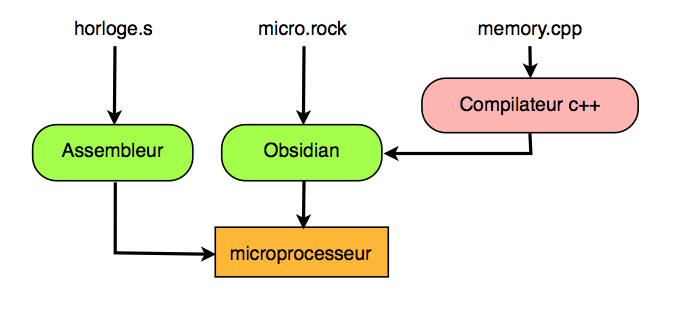
\includegraphics[width=13.5cm,height=6.2cm]{exec.png}
\caption{Architecture d'Obsidian}
\label{Architecture d'Obsidian}
\end{figure}

\end{document}
